\section{Project Overview}

\begin{frame}
	\begin{figure}[t]
		\centering
		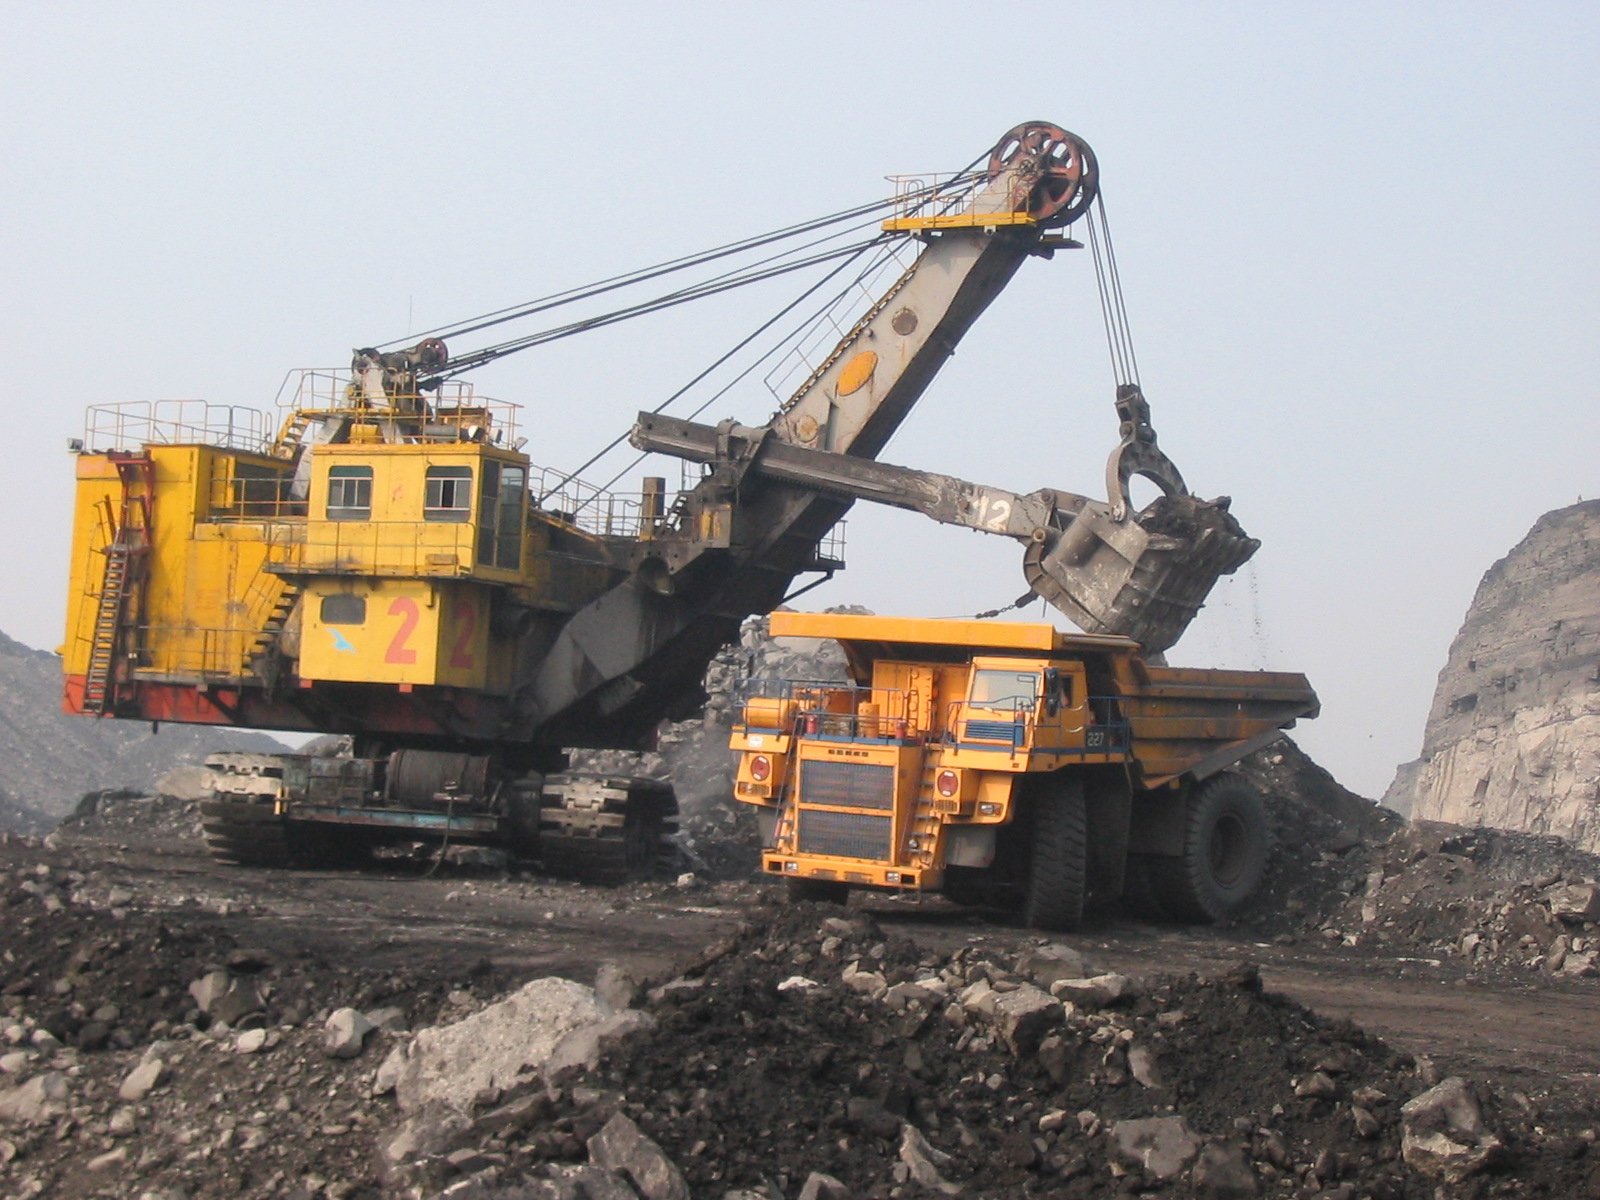
\includegraphics[width=.6\linewidth]{img/Excavator} \\
		\tiny{originally posted to Flickr by FAndrey at http://flickr.com/photos/43301444@N06/4141786255}
	\end{figure}

	\begin{itemize}
		\item{Goal: \textbf{Optimization of model parameters}}
		\item{Models of technical system = Physical properties + Control properties}
	\end{itemize}
\end{frame}

\begin{frame}
	\frametitle{Problem Setting}
	\begin{figure}[bth]
		\centering
		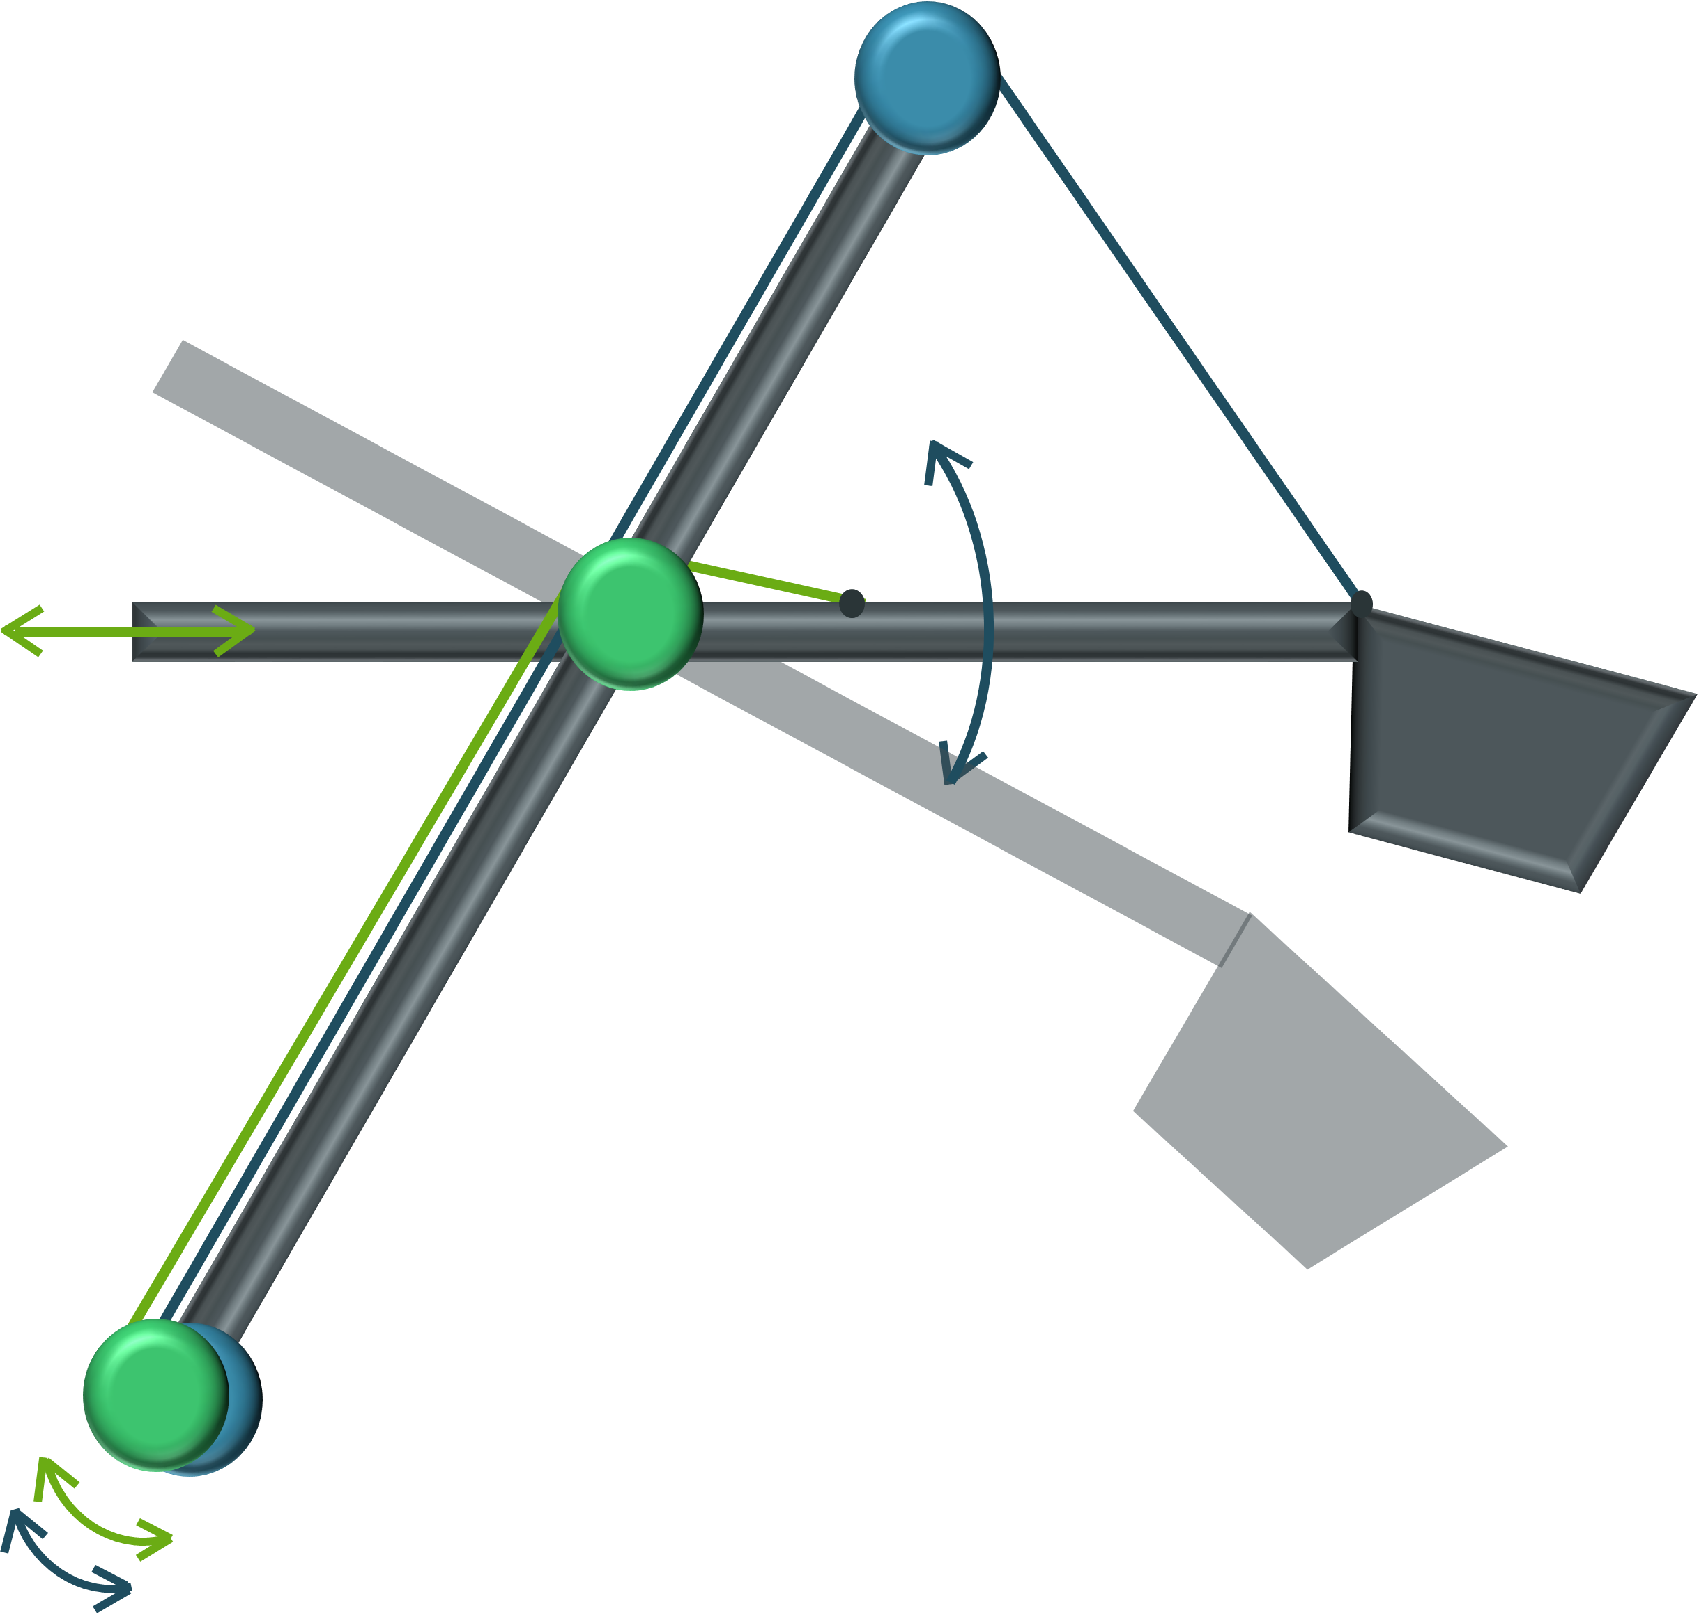
\includegraphics[width=.5\linewidth]{img/Problem_1}
	\end{figure}
\end{frame}

\begin{frame}
	\frametitle{Problem Setting}
	\begin{figure}[bth]
		\centering
		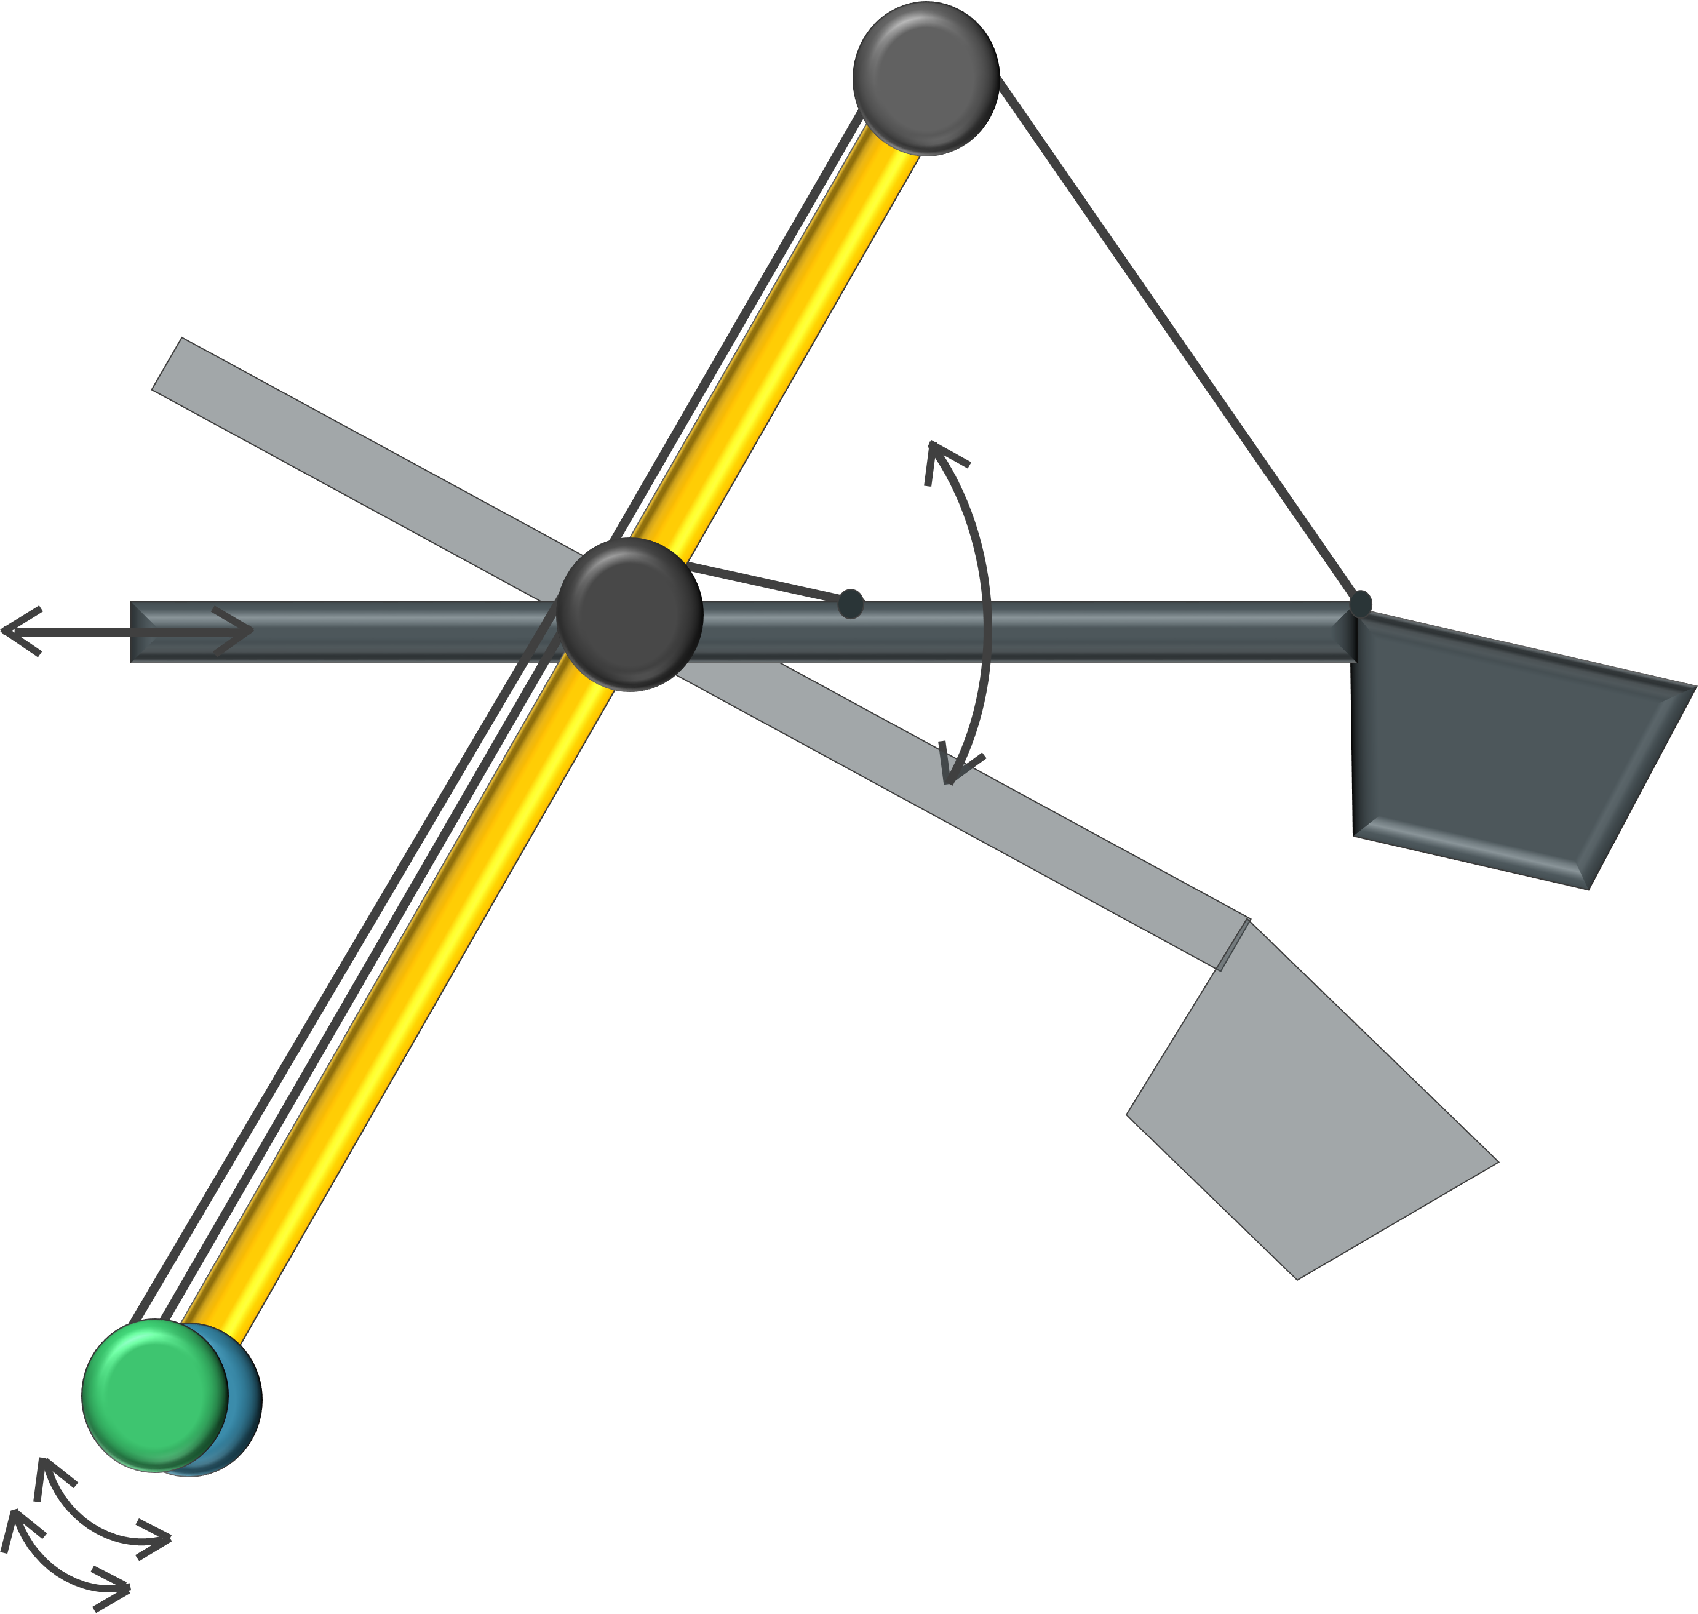
\includegraphics[width=.4\linewidth]{img/Problem_2}
	\end{figure}
	\begin{itemize}
		\item{Arm element fixed to the base}
		\item{Cannot be moved w.r.t. the base}
	\end{itemize}
\end{frame}

\begin{frame}
	\frametitle{Problem Setting (include videos)}
	\begin{figure}[bth]
		\centering
		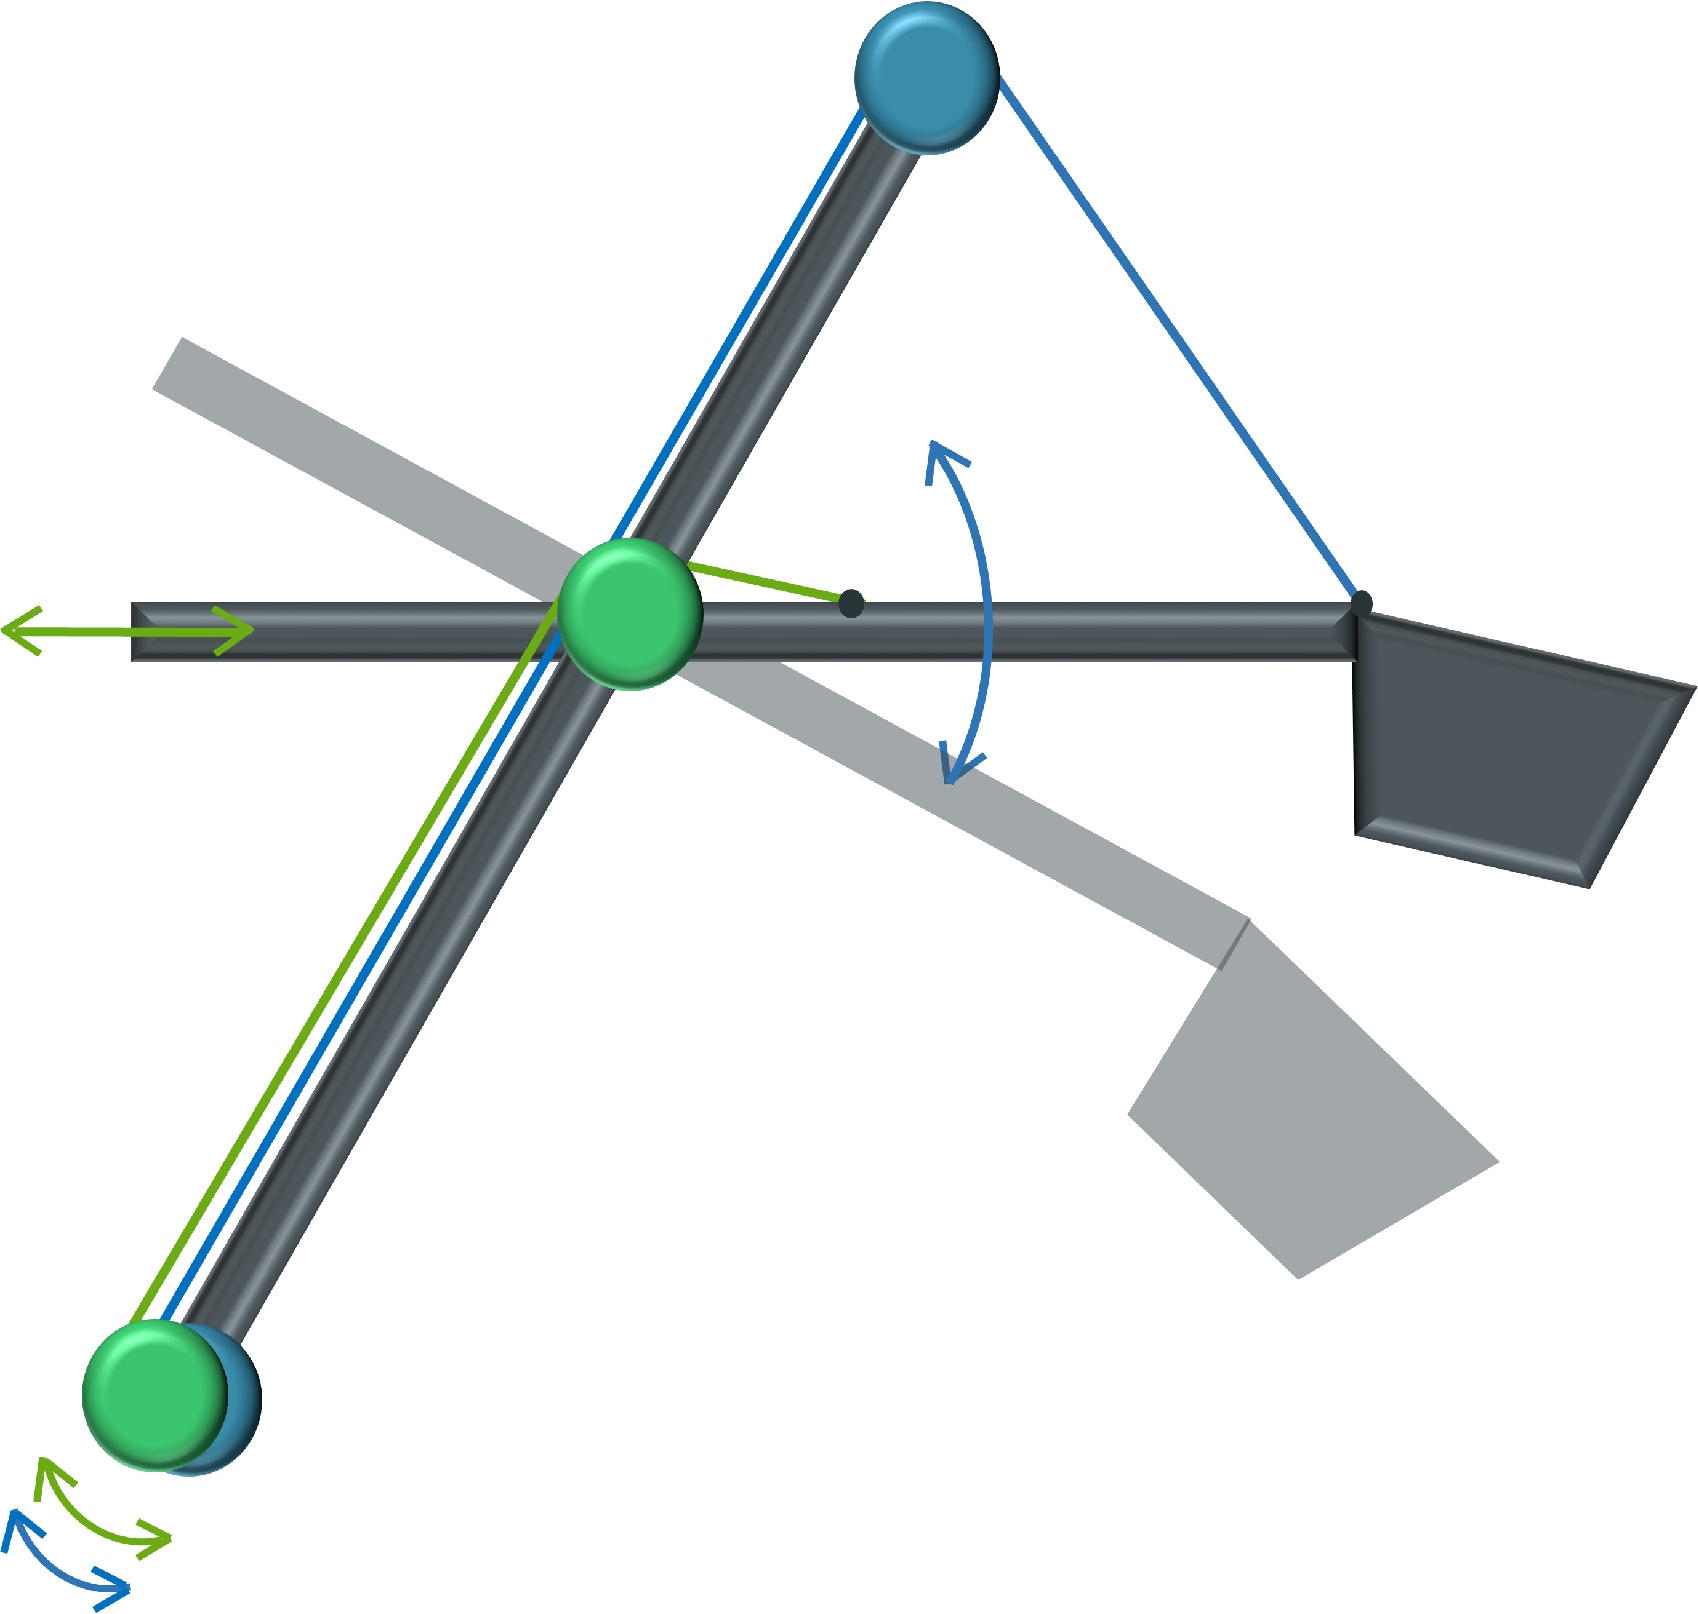
\includegraphics[width=.4\linewidth]{img/Problem_3}
	\end{figure}
	\centering
	\begin{itemize}
		\item{\makebox[1.5cm][l]{\textcolor[rgb]{0,0.69,0.32}{Green:}} Shovel motion \textbf{back} and \textbf{forth}}
		\item{\makebox[1.5cm][l]{\textcolor[rgb]{0.18,0.46,0.71}{Blue:}} Shovel motion \textbf{up} and \textbf{down}} \\
	\end{itemize}
\end{frame}


\begin{frame}
    \frametitle{Procedure}
    \onslide<1->
    \begin{columns}[onlytextwidth]
        \begin{column}{0.4\textwidth}
            \begin{block}{Physical Model}
                \begin{itemize}
                    \item{Rope properties}
                    \item{Lagrange Formalism}
                \end{itemize}
            \end{block}
            
            $\Downarrow$
            
            \begin{block}{Parameter Identification}
            Discretization
            \end{block}
        \end{column}
        
    \onslide<2>
        
        \begin{column}{0.05\textwidth}
        \textbf{vs}
        \end{column}
        
        \begin{column}{0.4\textwidth}
            \begin{exampleblock}{Blackbox Model}
                \begin{itemize}
                    \item{Realistic model}
                    \item{Confidential information}
                \end{itemize}
            \end{exampleblock}
            
            $\Downarrow$
            
            \begin{exampleblock}{Parameter Identification}
            Derivative-free optimization
            \end{exampleblock}
        \end{column}
    \end{columns}
\end{frame}


\begin{frame}
\setbeamertemplate{blocks}[rounded][shadow=false]
    \frametitle{Physical Modeling}
    \vspace{0.3cm}
		\large\textbf{Why?}
		\vspace{1cm}
		\begin{columns}
			\column{.3\textwidth}
				\centering
		    	\begin{block}{}
		    	    \begin{center}
		    	    \vskip 4mm
					{\large Building an accurate model}
					\vskip 3mm
					\hspace*\fill
					\end{center}
				\end{block}
			\column{.1\textwidth}
				\centering
				\Huge{$\Rightarrow$}
			\column{.3\textwidth}
				\centering
				\begin{block}{}
				    \begin{center}
				    \vskip 2mm
					Good description of the effects of control and motion
					%\vskip
					\hspace*\fill
					\end{center}
				\end{block}
		\end{columns}
	\vspace{0.5cm}
\end{frame}
	
	
\begin{frame}
    \frametitle{Physical Modeling Cont'd}
    \large\textbf{How?}
    \vspace{1cm}
	    \begin{columns}
	    \column{0.45\textwidth}
	    \onslide<1->
		To consider:
		\vspace{0.25cm}
		\begin{itemize}
			\item{Friction in cable reels}
			\item{Deformation of ropes}
			\item{Potential/Kinetic energy}
			\item{etc}
		\end{itemize}
		
		\onslide<2>
		\column{0.1\textwidth}
		    \Huge{$\rightarrow$}
		\column{0.35\textwidth}
		\large\textcolor{red}{Lagrange Formalism}\newline
		{(2nd order ODE)}
	\end{columns}
\end{frame}

\begin{frame}
    \frametitle{Physical Modeling Visualization}
    Why is it important?\newline
    \vspace{1cm}
    Performance videos of two different loads
\end{frame}







\begin{frame}
	\frametitle{Which color do we want to use?}
	\begin{tcolorbox}[width=\linewidth,colback={TUMblue}]
		TUMblue
	\end{tcolorbox}
	\begin{tcolorbox}[width=\linewidth,colback={TUMblue1}]
		TUMblue1
	\end{tcolorbox}
	\begin{tcolorbox}[width=\linewidth,colback={TUMblue2}]
		TUMblue2
	\end{tcolorbox}
	\begin{tcolorbox}[width=\linewidth,colback={TUMblue3}]
		TUMblue3
	\end{tcolorbox}
	\begin{tcolorbox}[width=\linewidth,colback={TUMblue4}]
		TUMblue4
	\end{tcolorbox}
	\begin{tcolorbox}[width=\linewidth,colback={TUMblue5}]
		TUMblue5
	\end{tcolorbox}
\end{frame}











\begin{frame}
\setbeamertemplate{blocks}[rounded][shadow=false]
	\frametitle{Parameter Identification}
	\onslide<1->
		\large\textbf{What are parameters?}
		\vspace{0.2cm}
		\begin{itemize}
			\item{Friction coefficients}
			\item{Mass}
			\item{Inertia}
			\item{etc.}
		\end{itemize}
	\vspace{0.5cm}
	\onslide<2>
		\large\textbf{Why?}
		\begin{columns}
			\column{.3\textwidth}
				\centering
		    	\begin{block}{}
		    	    \begin{center}
		    	    \vskip 4mm
					 Accurate and realistic parameters
					\vskip 3mm
					\hspace*\fill
					\end{center}
				\end{block}
			\column{.1\textwidth}
				\centering
				\Huge{$\Rightarrow$}
			\column{.3\textwidth}
				\centering
				\begin{block}{}
				    \begin{center}
				    \vskip 2mm
					Better prediction and planning of motion
					%\vskip
					\hspace*\fill
					\end{center}
				\end{block}
		\end{columns}
	\vspace{0.5cm}
\end{frame}
		

\begin{frame}
    \frametitle{Parameter Optimization Visualization}
    Two videos carrying the same load, but one with a random motion and the other with optimized parameters
\end{frame}



		
		
\begin{frame}
    \frametitle{Parameter Identification Two Ways}
    \vspace{0.2cm}
    \textbf{Two independent models acquired,}\newline
    \textbf{two different computational approaches.}
    \vspace{0.5cm}
    \begin{columns}[onlytextwidth]
        \begin{column}{0.4\textwidth}
            \begin{block}{Physical Model}
                \begin{itemize}
                    \item{Rope properties}
                    \item{Lagrange Formalism}
                \end{itemize}
            \end{block}
            
            $\Downarrow$
            
            \begin{block}{Parameter Identification}
            Discretization
            \end{block}
        \end{column}
        
        \begin{column}{0.05\textwidth}
        \textbf{vs}
        \end{column}
        
        \begin{column}{0.4\textwidth}
            \begin{exampleblock}{Blackbox Model}
                \begin{itemize}
                    \item{Realistic model}
                    \item{Confidential information}
                \end{itemize}
            \end{exampleblock}
            
            $\Downarrow$
            
            \begin{exampleblock}{Parameter Identification}
            Derivative-free optimization
            \end{exampleblock}
        \end{column}
    \end{columns}
\end{frame}		
		

\begin{frame}
    \frametitle{Parameter Identification: Physical Model}
    \vspace{-1cm}
    \onslide<1->
    \begin{columns}[onlytextwidth]
        \begin{column}{0.5\textwidth}
            \begin{block}{Own Physical Model}
                
                    {Lagrange Formalism}
                    \small{{\begin{align*}
	                        &A(x,p)
	                \begin{pmatrix} 
	                \ddot{s} \\ \ddot{\theta} \\
	                \end{pmatrix}
	                = b(x,u,p)
                    \end{align*}}}
            \vspace{-0.3cm}   
            \end{block}
            \vspace{-0.1cm}
            
            $\Downarrow$
            
            \begin{block}{Parameter Identification}
            Discretization
            \small{\begin{align*}
                \min_{x,p} & & \frac{1}{2} \| \bar{x} - x \|^2 & & \\
            \end{align*}}
            \vspace{-1cm}
            \end{block}
            \vspace{-1.5cm}
        \end{column}
    
    \onslide<2>
    \begin{column}{0.45\textwidth}
        \begin{itemize}
            \vspace{0.6cm}
            \item{All the information needed for calibration is available}
            \vspace{0.3cm}
            \item{Runge-Kutta method of different orders for discretization}
            \vspace{0.3cm}
            \item{Parameter computation for}\newline{a given control and motion}
        \end{itemize}
    \end{column}    
    \end{columns}
\end{frame}        
        
        
        
        
        
        
        
        
\begin{frame}        
    \frametitle{Parameter Identification: Blackbox Model}
    
    \onslide<2>
    \begin{columns}[onlytextwidth]
        \begin{column}{0.5\textwidth}
        \begin{itemize}
            \item{Almost no information is available except input/output}
            \vspace{0.3cm}
            \item{Derivative-free optimization methods required}
            \vspace{0.3cm}
            \item{As a real-life complex system, only a few parameters are studied here}
        \end{itemize}
        \end{column}
    
    
    
    \onslide<1->
    \begin{column}{0.45\textwidth}
            \begin{exampleblock}{Siemens Blackbox Model}
                \begin{itemize}
                
                \item{\textbf{Input}: Joystick commands for up/down/back/forth}
                \item{\textbf{Output}: Position of the shovel}
                \end{itemize}
            \end{exampleblock}
            
            $\Downarrow$
            
            \begin{exampleblock}{Parameter Identification}
            Particle Swarm, Pattern Search, Genetic Algorithm, ...
            \end{exampleblock}
        \end{column}
      \end{columns}
\end{frame}
